\documentclass[a4paper, 10pt]{article}
\usepackage[utf8]{inputenc}
\usepackage{verbatim}
\usepackage{listings}
\usepackage{graphicx}
\usepackage{a4wide}
\usepackage{color}
\usepackage{amsmath}
\usepackage{amssymb}
\usepackage[dvips]{epsfig}
\usepackage[toc,page]{appendix}
\usepackage[T1]{fontenc}
\usepackage{cite} % [2,3,4] --> [2--4]
\usepackage{shadow}
\usepackage{hyperref}
\usepackage{titling}
\usepackage{marvosym }
\usepackage{physics}

\usepackage{subcaption}
\usepackage[noabbrev]{cleveref}
\usepackage{wasysym}
\usepackage{changepage}


\renewcommand{\topfraction}{.85}
\renewcommand{\bottomfraction}{.7}
\renewcommand{\textfraction}{.15}
\renewcommand{\floatpagefraction}{.66}
\renewcommand{\dbltopfraction}{.66}
\renewcommand{\dblfloatpagefraction}{.66}
\setcounter{topnumber}{9}
\setcounter{bottomnumber}{9}
\setcounter{totalnumber}{20}
\setcounter{dbltopnumber}{9}


\setlength{\droptitle}{-10em}   % This is your set screw

\setcounter{tocdepth}{2}

\lstset{language=c++}
\lstset{alsolanguage=[90]Fortran}
\lstset{basicstyle=\small}
\lstset{backgroundcolor=\color{white}}
\lstset{frame=single}
\lstset{stringstyle=\ttfamily}
\lstset{keywordstyle=\color{red}\bfseries}
\lstset{commentstyle=\itshape\color{blue}}
\lstset{showspaces=false}
\lstset{showstringspaces=false}
\lstset{showtabs=false}
\lstset{breaklines}
\title{FYS3150/4150 - Project 1\\
  Nummerical methods for solving Poisson's equation}
\author{Aram Salihi$^1$, Adam Niewelgowski$^1$ \& Jakob Borg$^2$\\
  \small $^1$Department of Physics, University of Oslo, N-0316 Oslo, Norway\\
  \small $^2$Department of Theoretical Astrophysics, University of Oslo, N-0316 Oslo, Norway}
\begin{document}
\maketitle
\begin{abstract}
  \begin{center}
    In this article we have chosen to study three different algorithms (
    Thomas algorithm, a tailored verison of the thomas alogorithm
    and the famous LU decomposisition) for solving poission equation. We wish to
    compare the speed and the precision  of these three methods.
    \\
    We found out that the LU decomposisition is siginificantly slower than other two algorithms when compared,
    and the precision
    \href{https://github.com/einrone/FYS4150/}{GIT repository.}\footnote{\url{https://github.com/einrone/FYS4150/}}
  \end{center}
\end{abstract}
\section{Introduction:} The Poission equation is one of the most important and
widely used differential equation in different field of sciences,
especially in physics (e.g arises when solving different potentials in theoretical physics).
\begin{align}
  \nabla^{2}u = f
  \label{possion equation}
\end{align}
There is few cases in science general that this equation can be solved analytically, but quite
often it is not solvable, therefore it is crucial to derive nummerical alogorithms which is
time efficient and precise with minimal error. By using dirichlet boundaries and discretizing (\ref{possion equation})
this can be turned into a simple linear algebra problem on the form:
\begin{align}
  A\mathbf{u} = \mathbf{f}
\end{align}
Where $A$ is a $N \times N$ tridiagonal matrix. We wish to investigate three different alogorithms
mentioned in the abstract to solve this linear algebra problem. This problem can easily be solved by
LU decomposisition but as we later find out, this algorithm turns out be very slow when increasing
the dimension of the matrix. Due to the nature of tridiagonal matrix a more time effiecient and more precise method can be derived.
The Thomas algorithm is a simple method which uses foward and backward Gaussian elimination.
We will first present the general Thomas algorithm, a tailored version and LU decomposisition. We will then
compare the result and time the time used when running $N$ iteration.
\section{Theoretical Model:}
\subsection{Discretizing Possion's equation:} For the sake of simplicity we will reduce Poisson equation to
a one dimensional problem on the form:
\begin{align}
  \dv[2]{u(x)}{x} = f(x) \: , \quad x \in (0,1)
\end{align}
By assuming that the function $v$ is a smooth function, we will be using a taylor approximation up to fourth degree
and a approximation for the second derivative can be derived:
\begin{align}
  \dv[2]{u}{x} \approx -\frac{2u(x) - u(x+h) - u(x-h)}{h^{2}} + \mathcal{O}(h^{2})
\end{align}
(See appendix for derivation)By discretizing the function $u(x_{i})$ to $u_{i}$ and defining the grid points as $x_{i} = ih$, where $h$ is defined to
be $h = 1/(N+1)$. The above approximation can be formulated as:
\begin{align}
  \dv[2]{u}{x} \approx  -\frac{2u_{i} - u_{i+1} - u_{i-1}}{h^{2}} + \mathcal{O}(h^{2})
\end{align}
By imposing Dirichlet boundaries $x_{0} = 0$ and $ x_{n+1} = 1$ we have that:
\begin{align}
  u(0) = u(1) \to u_{0} = u_{n+1} = 0
\end{align}
Using this approximation and substituting this into Poissons equation, we will
then have:
\begin{align}
  -\frac{2u_{i} - u_{i+1} - u_{i-1}}{h^{2}} = f_{i}
\end{align}
where $f_{i} = f(x_{i})$ for $i = 1,...,n$.
Using the imposed conditions we can turn this problem into a simple linear
algebra problem on the form:
\begin{align}
  A\mathbf{u} = \mathbf{f}
\end{align}
where $\mathbf{u} = \{u_{1},.....,u_{n}\}$,
$\tilde{\mathbf{f}} = h^{2}\{f_{1},.....,f_{n}\}$ and $A$ is a $n\times n$ tridiagonal matrix on the form:
\begin{align}
  A = \begin{pmatrix}
    2 & -1 &0&.&.& 0\\
    -1 & 2 &-1&.&.& .\\
    .& ... & ... & ...&.&.\\
    . & .& ... & ... & -1&0\\
    .& . & .& -1 & 2& -1\\
    0& . & .& 0& -1& 2\\
  \end{pmatrix}
\end{align}
As we see the triadiagonal matrix has $2$ along its diagonal elements and $-1$ on the upper and
lower diagonal elements and has otherwise $0$ on the matrix elements.
\subsection{Solving a general tridiagonal problem (deriving Thomas algorithm):}
Recall the tridiagonal matrix from the previous section, we will now introduce a
general $n\times n$ tridiagonal matrix on the form:
\begin{align}
  A\mathbf{u} = \tilde{\mathbf{f}} \qquad \to \qquad
  \begin{pmatrix}
    b_{1} & c_1 & 0 & \ldots &  \ldots & 0\\
    a_1 & b_2 & c_2  & 0 & \ldots & 0\\
    0 & a_2 & b_3 &c_3 & 0 & \ldots \\
    0 & 0 & a_3 & b_4 &c_4 &\ldots\\
    \vdots &  & &  &\ddots & \vdots \\
    0 && \ldots && a_{n-1}&  b_n  \\
  \end{pmatrix}\begin{pmatrix}
    u_1\\
    u_2\\
    u_3\\
    u_4\\
    \vdots\\
    u_n\\
  \end{pmatrix}=
  \begin{pmatrix}
    s_1\\
    s_2\\
    s_3\\
    s_4\\
    \vdots\\
    s_n
  \end{pmatrix}
\end{align}
In order to solve this equation we must
perform a forward and a backward substitution. By performing Gaussian elimination on the second row in order to get a pivot coloumn, we must
multiply the first row with $a_{1}/b_{1}$ and substract the first row with the second row. This will give us the matrix:
\begin{align}
  \begin{pmatrix}
    b_{1} & c_1 & 0 & \ldots &  \ldots & 0\\
    0 & d_{2} & c_2  & 0 & \ldots & 0\\
    0 & a_2 & b_3 &c_3 & 0 & \ldots \\
    0 & 0 & a_3 & b_4 &c_4 &\ldots\\
    \vdots &  & &  &\ddots & \vdots \\
    0 && \ldots && a_{n-1}&  b_n  \\
  \end{pmatrix}\begin{pmatrix}
    u_1\\
    u_2\\
    u_3\\
    u_4\\
    \vdots\\
    u_n\\
  \end{pmatrix}=
  \begin{pmatrix}
    \tilde{f}_{1}\\
    s_2\\
    \tilde{f}_{3}\\
    \tilde{f}_{4}\\
    \vdots\\
    \tilde{f}_{n}
  \end{pmatrix}
\end{align}
Where we have defined $d_{2}$ and $s_{2}$ to be:
\begin{align}
  d_{2} = b_{2} - c_{1}\frac{a_{1}}{b_{1}} \qquad s_{2} = \tilde{f}_{2} - \tilde{f}_{1}\frac{a_{1}}{b_{1}}
\end{align}
By repeating this procudere we will see a pattern, and the foward substitution is
derived to be\\ (if we define a initial conditon, $d_{1} = b_{1}$ and $\tilde{f}_{1} = s_{1}$):
\begin{align}
  d_{i} = b_{i} - c_{i-1}\frac{a_{i-1}}{d_{i-1}}
  \qquad
  s_{i} = \tilde{f}_{i} - s_{i-1}\frac{a_{i-1}}{d_{i-1}}
\end{align}
We have now successfully produced pivot elements
on every coloumns in the matrix.
\begin{align}
  \begin{pmatrix}
    d_{1} & c_1 & 0 & \ldots &  \ldots & 0\\
    0 & d_{2} & c_2  & 0 & \ldots & 0\\
    0 & 0& d_3 &c_3 & 0 & \ldots \\
    0 & 0 & 0 & d_4 &c_4 &\ldots\\
    \vdots &  & &  &\ddots & \vdots \\
    0 && \ldots && 0 &  d_{n} \\
  \end{pmatrix}\begin{pmatrix}
    u_1\\
    u_2\\
    u_3\\
    u_4\\
    \vdots\\
    u_n\\
  \end{pmatrix}=
  \begin{pmatrix}
    s_{1}\\
    s_2\\
    s_{3}\\
    s_{4}\\
    \vdots\\
    s_{n}
  \end{pmatrix}
\end{align}
The equations above can be iterated from $i = 1$ to $n$ and will give us the correct matrix elements
when its reduced to its row echelon form. In order to achieve the solution set $\mathbf{u}$ we must
perform a backward substitution. Consider following (written out the matrix equation):
\begin{align}
  b_{1}v_{1} + c_{1}v_{2} = s_{1}
  \\
  d_{2}v_{2} + c_{2}v_{3} = s_{2}
  \\
  .
  \\
  .
  \\
  .
  \\
  d_{n-1}u_{n-1} + c_{n-1}u_{n} = s_{n-1}
  \\
  d_{n}u_{n} = s_{n}
  \label{backward substitution}
\end{align}
If we look at the second last and last equation in (\ref{backward substitution})
and solve for $u_{n}$ and $u_{n-1}$ we have:
\begin{align}
  u_{n} = s_{n}/d_{n} \qquad u_{n-1} = \frac{s_{n-1} - u_{n}c_{n-1}}{d_{n-1}}
\end{align}
changing the dummy index $n$ to $j$ and using $u_{n} = s_{n}/d_{n}$ as the initial value when performing
backward substitution, the equation we obtain is:
\begin{align}
  u_{j-1} = \frac{s_{j-1} - u_{j}c_{j-1}}{d_{j-1}}
\end{align}
Where $j$ iterates from $j = n-1$ down to $j = 1$. Thus the general algorithm to solve
the general tridiagonal matrix problem is:
\paragraph{Foward substitution}
\begin{align}
  d_{i} = b_{i} - c_{i-1}\frac{a_{i-1}}{d_{i-1}}
  \qquad
  s_{i} = \tilde{f}_{i} - s_{i-1}\frac{a_{i-1}}{d_{i-1}} \qquad 1 \le i < N+1
\end{align}
\paragraph{Backward substitution}
\begin{align}
  u_{j-1} = \frac{s_{j-1} - u_{j}c_{j-1}}{d_{j-1}} \qquad  N-1 \le j \le 1
\end{align}
As we later see, this method turns out be a very efficient and precise algorithm
when comparing to LU-decomposisition.
\section{Optimizing Thomas algorithm for a special case:} It turns out that the previous
algorithm which is already quite fast can be modified to a faster algorithm. Recall from
previous that the diagonal element had values $a_{1},...,a_{n-1}$,
$b_{1},...,b_{n-1}$ and $c_{1},...,c_{n-1}$ where we assumed that none of these values were the same to keep it general.
We will now define that:
\begin{align}
  a_{1},...,a_{n-1} = -1
  \\
  b_{1},......,b_{n-1} = 2
  \\
  c_{1},...,c_{n-1} = -1
\end{align}
By doing this we can rewrite our general algorith to fit this specific case:
(må forklare nede hvordan man ser at d blir sånn):
\paragraph{Foward substitution}
\begin{align}
  d_{i} = \frac{i + 1}{i} 
  \qquad
  s_{i} = \tilde{f}_{i} + \frac{s_{i-1}}{d_{i-1}} \qquad 1 \le i < N+1
\end{align}
\paragraph{Backward substitution}
\begin{align}
  u_{j-i} = \frac{s_{j-1}+u_{j}}{d_{j-1}} \qquad  N-1 \le j \le 1
\end{align}

This operation reduces number of FLOPS (see section LATER LOOL - der vi skal
beregne dette i diskusjon) for each calculation what makes algorithm more
effective.

SKAL vi skrive om LU eller bare gi formelen og hvoran det funker og gi kilde
til bevis og sånt? og ellers nøye oss med resultater og diskusjon
om presisjon og hastighet hovedsakelig?

\section{Method:}
Every algorithm listed below is implemented in C++. Armadillo library is used
in LU-decomposition.
\subsection{General algorithm:}
As derived above in section (GIVE SECTION), Thomas algorithm has two loops,
forward and backward substitution 
\begin{lstlisting}
//forward
for(int i = 2; i <= N+1; i++){
        b[i] -= (a[i-1]*c[i-1])/b[i-1];
        s[i] -= s[i-1]*(a[i-1]/b[i-1]);
    }
//backward
v[N-1] = s[N-1]/b[N-1]; //initial - last element
for(int i = N+1; i > 1; i--){
        v[i-1]= (s[i-1] - c[i-1]*v[i])/b[i-1];
    }
\end{lstlisting}
we notice that  the algorithm is for the general use where every value of matrix
elements can be different.
\subsection{Specific algorithm:}
Implementation of the algorithm for the specified matrix is as follows
\begin{lstlisting}
//forward
    for(int i = 1; i <= N+1; i++){
        b[i] = (i+1.0)/((double)i);
        s[i] += s[i-1]/(b[i-1]);
    }
//backward
    v[N-1] = s[N-1]/b[N-1]; //initial - last element
    for(int i = N+1; i > 1; i--){
        v[i-1] = (s[i-1] + v[i])/b[i-1];
    }
\end{lstlisting}
algorithm still needs to run through two loops with a few operations, but we
can clearly see the simplicity of this algorith compared with general one.
\subsection{LU-decomposition:}
For calculation with LU-decomposition, we need first to implement
initialization of the matrix A
\begin{lstlisting}
	LU - matrise A
\end{lstlisting}
then we can use lu and solve module to find the solution
\begin{lstlisting}
	kode med lu og solve
\end{lstlisting}
\subsection{Precision:}
To be able to say something about accuracy of the numerical solution, we can
calculate the relative error given by
\begin{align*}
  \epsilon_{i} = \log_{10}\left(\mid \frac{v_{i}-u_{i}}{u_{i}} \mid \right)
\end{align*}
where \(u_{i}\) is the discretized exact solution and \(v_{i}\) is the
simulated solution.
\section{Results:}
\begin{figure}[H]
  \centering
  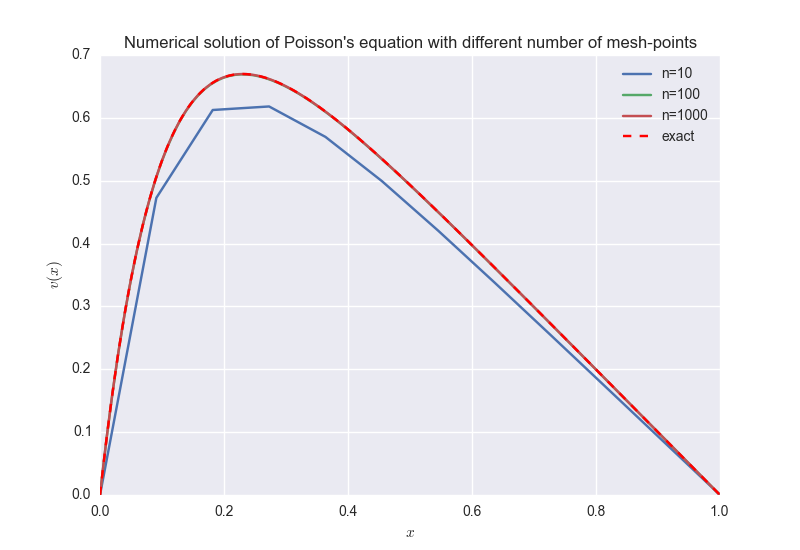
\includegraphics[width= 12cm]{simulation_general.png}
  \caption{Plot of simulated solution compared with the exact function}
  \label{fig:Figure 1} 
\end{figure}



bilder av løsningen og error, vi kan prøve å plotte LU error sammen med
gaussian error i en for å se om det er noen forskjell der
-beskrive hvorfor feilen øker igjen og hvorfor den faller som den gjør, med
stigningstallet 2 i log-log plot

lage tabell med tidene og diskutere dette med flops og beregne de



\end{document}
